\documentclass[tikz,border=4pt]{standalone}
\usepackage{tikz}
\usepackage{amsmath}
\usepackage{amssymb}
\usetikzlibrary{decorations.pathreplacing,positioning}

\begin{document}
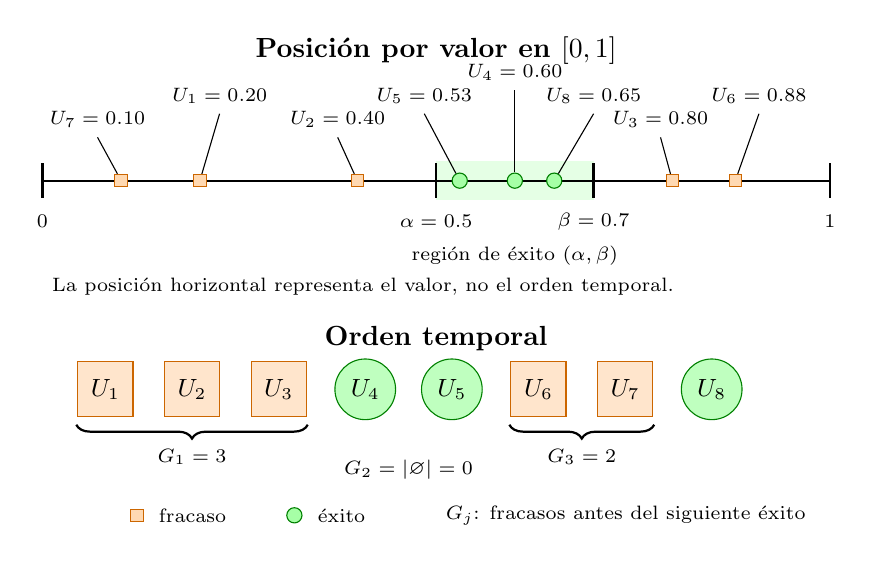
\begin{tikzpicture}[
    value failure/.style={draw=orange!80!black,fill=orange!30,rectangle,
        minimum size=4.5pt,inner sep=1pt},
    value success/.style={draw=green!50!black,fill=green!35,circle,
        minimum size=5.5pt,inner sep=1pt},
    time failure/.style={draw=orange!80!black,fill=orange!20,rectangle,
        minimum width=7mm,minimum height=7mm,font=\small},
    time success/.style={draw=green!50!black,fill=green!25,circle,
        minimum size=7mm,font=\small},
    small label/.style={font=\scriptsize}
]
    \node[font=\bfseries] at (5,4.85) {Posición por valor en $[0,1]$};
    \fill[green!10] (5,2.95) rectangle (7,3.45);
    \draw[thick] (0,3.2) -- (10,3.2);
    \foreach \x/\lab in {0/0,5/{\alpha=0.5},7/{\beta=0.7},10/1} {
        \draw[thick] (\x,3.42) -- (\x,2.98);
        \node[small label] at (\x,2.68) {$\lab$};
    }
    \node[small label] at (6,2.25) {región de éxito $(\alpha,\beta)$};

    \node[value failure] (v1) at (2,3.2) {};
    \draw[thin] (v1) -- (2.25,4.05) node[above,small label] {$U_1=0.20$};
    \node[value failure] (v2) at (4,3.2) {};
    \draw[thin] (v2) -- (3.75,3.75) node[above,small label] {$U_2=0.40$};
    \node[value failure] (v3) at (8,3.2) {};
    \draw[thin] (v3) -- (7.85,3.75) node[above,small label] {$U_3=0.80$};
    \node[value success] (v4) at (6,3.2) {};
    \draw[thin] (v4) -- (6,4.35) node[above,small label] {$U_4=0.60$};
    \node[value success] (v5) at (5.3,3.2) {};
    \draw[thin] (v5) -- (4.85,4.05) node[above,small label] {$U_5=0.53$};
    \node[value failure] (v6) at (8.8,3.2) {};
    \draw[thin] (v6) -- (9.1,4.05) node[above,small label] {$U_6=0.88$};
    \node[value failure] (v7) at (1,3.2) {};
    \draw[thin] (v7) -- (0.7,3.75) node[above,small label] {$U_7=0.10$};
    \node[value success] (v8) at (6.5,3.2) {};
    \draw[thin] (v8) -- (7,4.05) node[above,small label] {$U_8=0.65$};
    \node[small label,anchor=west] at (0,1.85)
        {La posición horizontal representa el valor, no el orden temporal.};

    \node[font=\bfseries] at (5,1.2) {Orden temporal};
    \foreach \i/\x in {1/0.8,2/1.9,3/3.0} {
        \node[time failure] (t\i) at (\x,0.55) {$U_{\i}$};
    }
    \node[time success] (t4) at (4.1,0.55) {$U_4$};
    \node[time success] (t5) at (5.2,0.55) {$U_5$};
    \node[time failure] (t6) at (6.3,0.55) {$U_6$};
    \node[time failure] (t7) at (7.4,0.55) {$U_7$};
    \node[time success] (t8) at (8.5,0.55) {$U_8$};

    \draw[decorate,decoration={brace,amplitude=5pt,mirror},thick]
        (0.43,0.10) -- (3.37,0.10)
        node[midway,below=5pt,small label] {$G_1=3$};
    \node[small label] at (4.65,-0.47) {$G_2=\lvert\varnothing\rvert=0$};
    \draw[decorate,decoration={brace,amplitude=5pt,mirror},thick]
        (5.93,0.10) -- (7.77,0.10)
        node[midway,below=5pt,small label] {$G_3=2$};

    \node[value failure] (legend-failure) at (1.2,-1.05) {};
    \node[small label,right=2pt of legend-failure] {fracaso};
    \node[value success] (legend-success) at (3.2,-1.05) {};
    \node[small label,right=2pt of legend-success] {éxito};
    \node[small label,anchor=west] at (5,-1.05)
        {$G_j$: fracasos antes del siguiente éxito};

\end{tikzpicture}
\end{document}
